% !TeX spellcheck = en_GB 

\section{\label{sec::results}Results}

In the following we want to show some results of our simulations. If not explicitly mentioned, we use the properties described in section \ref{sec::modelling}.

The first thing we have a closed look at, is a constant Dirichlet boundary. With this we can model an oven with relatively fast circulating air, so the outermost layer is always covered with hot air. In figure \ref{fig::dirichlet2D} we can see the heating progress of this model. Interesting to notice is, that the aluminium stick is almost completely heated to $200\SI{}{\degreeCelsius}$ after one minute. From physical perspective this is not suprising since the factor between $\alpha_{cake}$ and $\alpha_{Al}$ is aproximately $10^2$.

As people tend to be impatient, it might also be interesting, to consider the case, in which we heat up the oven, while the cake is already in it. This is modelled by time dependent Dirichlet conditions. For the example in figure \ref{fig::dirichletHeat2D} we heat up the oven quite slowly, so the effect can be seen better. Of course the average temperature in this case rises slower. Compared to the constant boundary the average and the minimal temperature stay closer together here. We are not experts in baking, but maybe there are situations, where this is an advantage.

In the previous examples we saw, how the aluminium rod in the middle heated up the cake from the inside. To see, how much influence on the baking progress it actually had, we modelled the whole process without the aluminium in figure \ref{fig::dirichletFull2D} and replaced it with dough. During the first 40 minutes the middle of the cake almost does not heat up at all. In total it takes almost three hours for the cake to be done\footnote{Experience reports, which can be found in cooking forums, lead to the speculation of cake being done at approximately 93\SI{}{\degreeCelsius}.} in the middle.\\

In all of our tested cases the cake takes pretty long to be finished. Most likely most of them would be burned from the outside, before being done in the middle.\footnote{In practice professionals never bake such big massive cakes at ones. My room-mate back home, who is a confectioner, told me that cakes like this are baked in layers and putted together afterwards.} Considering this, our work might not exactly help to improve ones baking performance, but it definitely gives a nice intuition, of how the heat equation can be modelled with the help of finite elements and an appropriate ODE-solver.

\newpage
\section*{Appendix}

\begin{figure}[htp]
        \centering
        \makebox[\textwidth][c]{
        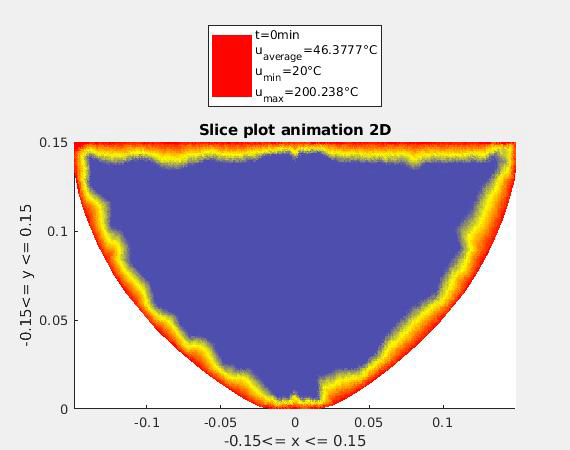
\includegraphics[width=0.69\textwidth]{figures/dirichlet_200_2D001.png}
        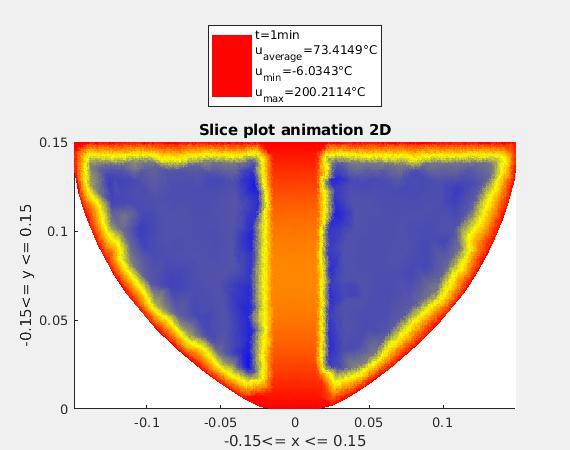
\includegraphics[width=0.69\textwidth]{figures/dirichlet_200_2D002.png}
        }
        \makebox[\textwidth][c]{
        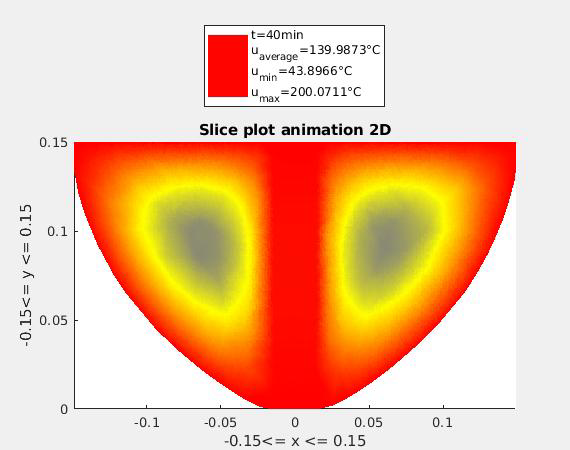
\includegraphics[width=0.69\textwidth]{figures/dirichlet_200_2D041.png}
        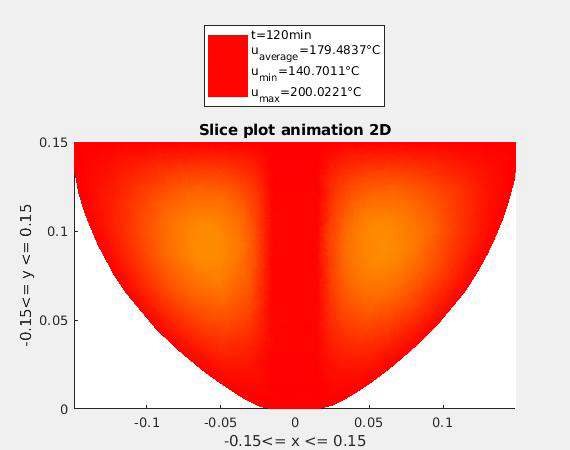
\includegraphics[width=0.69\textwidth]{figures/dirichlet_200_2D121.png}
        }
        \caption{\label{fig::dirichlet2D} side view of 200\SI{}{\degreeCelsius} Dirichlet boundary}
\end{figure}

\begin{figure}[htp]
        \centering
        \makebox[\textwidth][c]{
        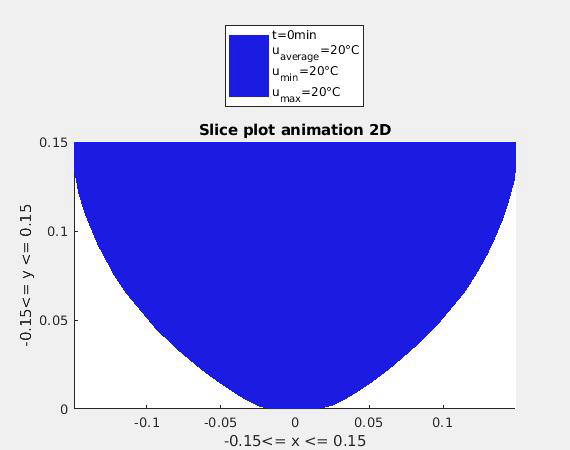
\includegraphics[width=0.69\textwidth]{figures/dirichlet_heat_200_2D001.png}
        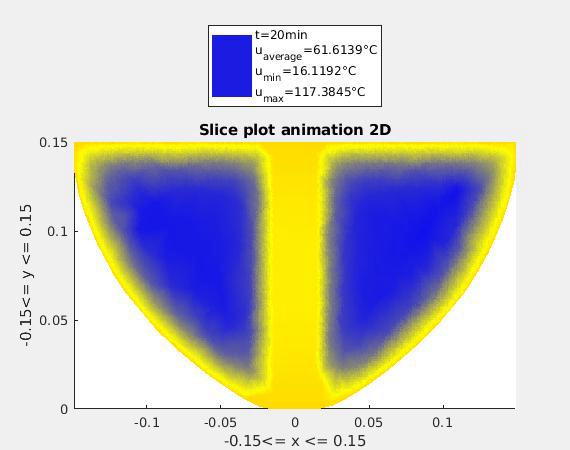
\includegraphics[width=0.69\textwidth]{figures/dirichlet_heat_200_2D021.png}
        }
        \makebox[\textwidth][c]{
        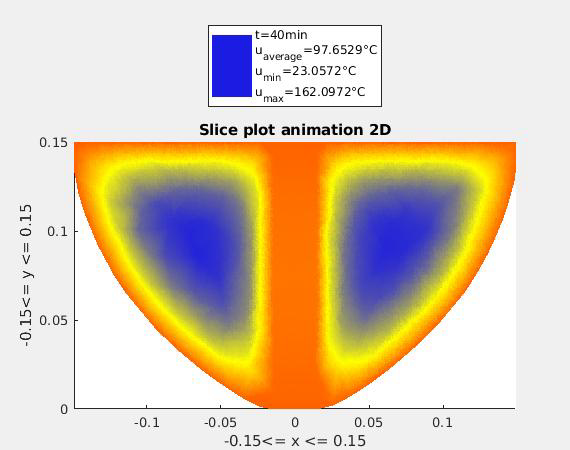
\includegraphics[width=0.69\textwidth]{figures/dirichlet_heat_200_2D041.png}
        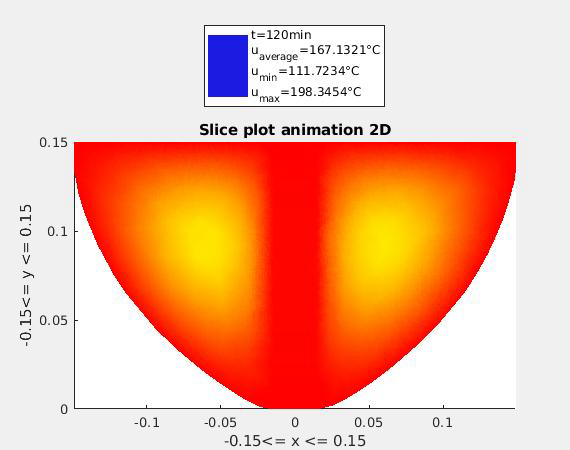
\includegraphics[width=0.69\textwidth]{figures/dirichlet_heat_200_2D121.png}
        }
        \caption{\label{fig::dirichletHeat2D} side view heating Dirichlet boundary boundary}
\end{figure}

\begin{figure}[htp]
        \centering
        \makebox[\textwidth][c]{
        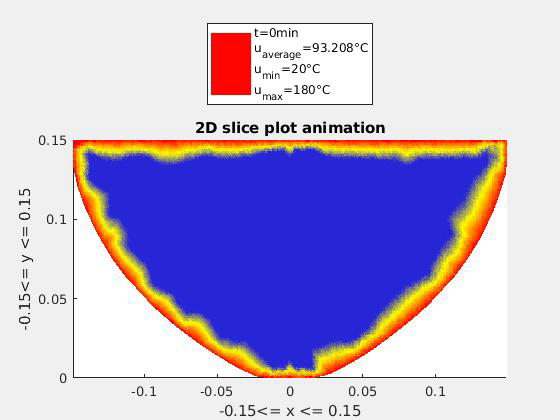
\includegraphics[width=0.69\textwidth]{figures/dirichlet_fullCake_2D001.png}
        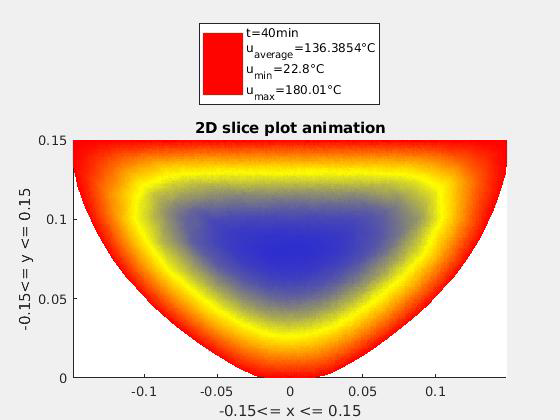
\includegraphics[width=0.69\textwidth]{figures/dirichlet_fullCake_2D041.png}
        }
        \makebox[\textwidth][c]{
        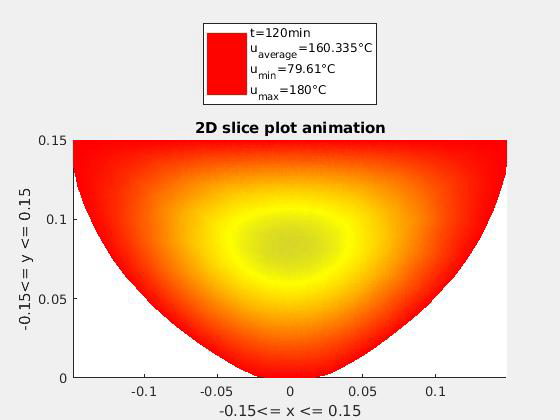
\includegraphics[width=0.69\textwidth]{figures/dirichlet_fullCake_2D121.png}
        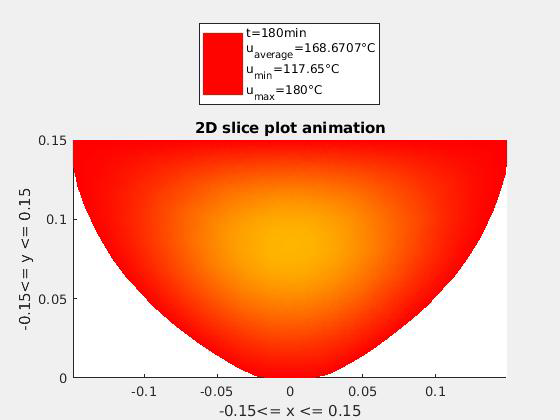
\includegraphics[width=0.69\textwidth]{figures/dirichlet_fullCake_2D181.png}
        }
        \caption{\label{fig::dirichletFull2D} side view of a baking cake without the aluminium stick}
\end{figure}
